\chapter{The Universe}

    Rise does not attempt to define a single geography with specific countries and locations that is shared between all games.
    It is common for GMs to define their own setting when running a game, and that freedom is important.
    However, the universe of Rise does differ in a number of important ways from the real world.
    The fundamental assumptions that Rise makes about the world are listed below.
    These fundamental elements are ambiguous about some details, and GMs are encouraged to fill in those details as they see fit.
    Of course, a GM has absolute power, and can create a world that changes any number of these assumptions.
    However, doing so can significantly change the tone of the game and create logical inconsistencies, so it should be done carefully.

\section{Magic is Common}
    The world of Rise is a magical place.
    Many people are capable of using magic to perform feats that would be impossible in the real world.
    Not everyone is capable of magic, of course.
    As an overly broad generalization, it's reasonable to assume that about a quarter of the civilized people in the world have some ability to use magic.
    In some societies, such as a feudal human-dominated society with a large number of commoners and serfs, the percentage of people with magic can be much lower.
    However, this is balanced by the existence of other societies that tend to be much more magical, such as societies ruled by gnomes and elves.
    Even in low-magic societies, everyone knows that magic exists, and almost everyone has observed or been personally affected by magic at some point in their lives.

    People can have magical abilities for a wide variety of reasons.
    There are three main categories to explain why people can access magic: intrinsic magic, learned magic, and gifted magic.
    Each class with magical abilities belongs to one of these groups.
    Characters with magical feats are free to choose any of those three explanations for their feats.
    The explanation does not have to be the same as for any other magical abilities they possess.
    For example, a cleric may be gifted their magical cleric abilities because they worship a particular deity, but they may also be naturally telepathic.

    Some people are simply intrinsically magical.
    They may require training and experience to improve their natural magical talents, but they had magical capabilities before doing any training.
    This intrinsic magic can come from magical ancestry, unusual birth circumstances, magical experimentation, exposure to powerful magic, simple random chance, or any number of other sources.
    This is the standard explanation for sorcerers.
    In addition, this is the most common explanation for the magical abilities of monsters.

    Some people gain access to magic through personal training or research.
    These people find ways to tap into some pre-existing magical property of the universe and manipulate it at their command.
    This is the standard explanation for monks, rangers with the Beastmaster archetype, rogues with the Bardic Music archetype, and wizards.

    Some people are gifted magic by their association with powerful magical entities or forces.
    They offer worship, allegiance, or their souls, and are granted magical power in exchange.
    This is the standard explanation for clerics, druids, paladins, and warlocks.

\section{Personal Power Comes From Great Deeds}
    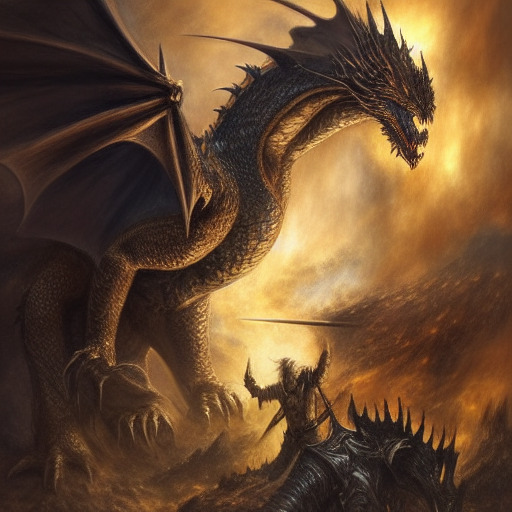
\includegraphics[width=\columnwidth]{the universe/great deeds}
    The average person in the world of Rise is not particularly more or less capable than the average person in the real world.
    Training can help people improve their skills, but as in the real world, anyone who tries to improve themselves through training and practice eventually reaches an upper limit to their potential.
    However, unlike in the real world, people in Rise can reach beyond their ordinary limitations.
    By defeating powerful foes and performing great deeds that influence the world around them, people can gain levels, which allows them to reach new heights of power.
    At high levels, people can perform clearly superhuman feats that would be impossible for ordinary humans, even without the influence of magic.

    People in Rise wouldn't usually talk about "levels" as a discrete concept ranging from 1 to 21.
    They would perceive the world as a spectrum, and the specific divisions would be more subtle.
    However, they would be aware that some people are fundamentally stronger and more skilled than others.
    Individual scholars or scholastic groups may create their own concepts in-universe to categorize and explain the phenomenon of levels, since the growth of personal power over time is observable and studiable. 
    However, those in-universe concepts would never exactly replicate the metagame concept of a level.

    It is common for people in positions of political power to also wield unusually large amounts of personal power.
    High level individuals can be savvier, wiser, and more persuasive than any ordinary human.
    They are more likely than low-level individuals to be able to gain political power through whatever means they see fit, and more likely to maintain their hold on that power.
    In addition, political power can grant further opportunities for performing great deeds, which helps those in power to gain levels and stay ahead of any competition.

    The fastest path to acquiring personal power does not come from pursuing political power.
    It comes from adventuring.
    Adventurers can defeat powerful monsters, help towns in need, and otherwise have a significant personal influence on the world.
    In the process of these adventures, they can amass personal power much more rapidly than ordinary people.
    Of course, adventuring also has an unusually high risk of death.
    Even worse, people who die while adventuring often leave their corpse in the middle of nowhere - in a monster's stomach - which prevents them from being resurrected without incredibly rare magic.
    Adventurers must constantly seek out new challenges to test their limits, or else they will stagnate and stop acquiring personal power, so it is never a sustainable long-term activity.
    There are many people in the world who were adventurers at some point in their past, and everyone is familiar with the concept, but active adventurers are still unusual.

\section{Deities and Afterlifes}\label{Deities and Afterlifes}
    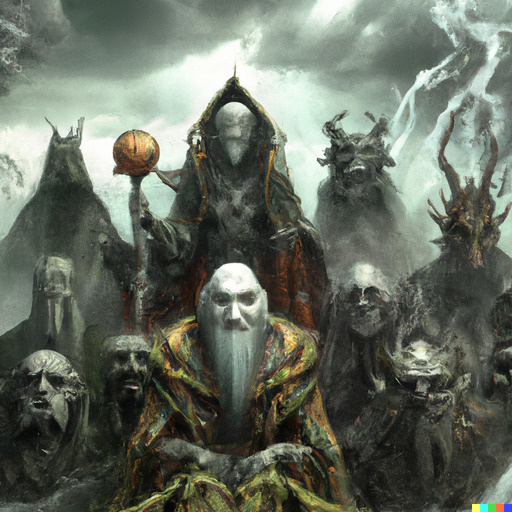
\includegraphics[width=\columnwidth]{the universe/deities and afterlifes}

    When a humanoid creature dies in Rise, they know beyond a shadow of a doubt that they will go to an afterlife.
    Most likely, they know exactly which afterlife they will go to, either as a result of their alignment or their worship of a particular deity.
    In that afterlife, they will live again for as long as they want, though they cannot leave without being magically resurrected.
    People are confident that this is true because deities have told them so, and deities are provably real.
    Also, rare and powerful magic can be used to communicate with people in their afterlife, or even to physically travel to an afterlife plane.

    It is an undisputed fact that Rise is filled with a wide variety of deities of varying power and influence.
    They divinely empower their clerics to act on their behalf.
    Many people know, though some chain of connections, someone who chose to become a cleric and was quickly rewarded with divine magic far beyond anything they could previously do on their own.
    Everyone has heard legends of deities intervening more directly in the world even without a cleric, though these stories are rare and few have experienced them firsthand.

    There are nine distinct afterlife planes, with one plane for each alignment combination.
    Each of those planes is divided into layers.
    Some of those layers are reserved for deities, with major deities claiming layers that are entirely their own and multiple minor deities sharing territory within a single layer.
    The remaining layers have no specific associated deity.
    People can travel between the layers, though the specific mechanisms for traversing layers are different for each afterlife plane.
    Most people do not know this level of detail about afterlife planes, and a commoner would simply be confident that they will go where they belong.

    It is well known that the afterlife planes for evildoers are much harsher than the other afterlife planes.
    The three evil afterlife planes are collectively referred to the Abyss.
    Demons stalk those planes, tormenting evildoers for their own sadistic reasons.
    One of the reasons that some people worship evil deities is to gain a promise of safety, since evil deities protect their worshippers from demonic torment in the afterlife.
    It is also said that demons only torment the weak-willed, and that those who escape demonic torments are free to live in hedonistic luxury.
    There is truth in this, though there are far more people who are confident that they would rule proudly in the Abyss than people who succeed.

    A list of specific well-known deities is given in \trefnp{Deities}.
    Of course, the GM may introduce new major deities, and the many minor deities worshipped by monsters are not listed here.

    \begin{dtable!*}
        \lcaption{Deities}
        \begin{dtabularx}{\textwidth}{X l X}
            \tb{Deity} & \tb{Alignment} & \tb{Domains} \tableheaderrule
            Gregory, warrior god of mundanity     & Lawful good     & Law, Protection, Strength, War         \\
            Guftas, horse god of justice          & Lawful good     & Good, Law, Strength, Travel            \\
            Lucied, paladin god of justice        & Lawful good     & Destruction, Good, Protection, War     \\
            Simor, fighter god of protection      & Lawful good     & Good, Protection, Strength, War        \\
            Ayala, naiad god of water             & Neutral good    & Life, Magic, Water, Wild               \\
            Pabs Beerbeard, dwarf god of drink    & Neutral good    & Good, Life, Strength, Wild             \\
            Rucks, monk god of pragmatism         & Neutral good    & Good, Law, Protection, Travel          \\
            Vanya, centaur god of nature          & Neutral good    & Good, Strength, Travel, Wild           \\
            Brushtwig, pixie god of creativity    & Chaotic good    & Chaos, Good, Trickery, Wild            \\
            Camilla, tiefling god of fire         & Chaotic good    & Fire, Good, Magic, Protection          \\
            Chavi, wandering god of stories       & Chaotic good    & Chaos, Knowledge, Trickery             \\
            Chort, dwarf god of optimism          & Chaotic good    & Good, Life, Travel, Wild               \\
            Ivan Ivanovitch, bear god of strength & Chaotic good    & Chaos, Strength, War, Wild             \\
            Krunch, barbarian god of destruction  & Chaotic good    & Destruction, Good, Strength, War       \\
            Sir Cakes, dwarf god of freedom       & Chaotic good    & Chaos, Good, Strength                  \\
            Mikolash, scholar god of knowledge    & Lawful neutral  & Knowledge, Law, Magic, Protection      \\
            Raphael, monk god of retribution      & Lawful neutral  & Death, Law, Protection, Travel         \\
            Declan, god of fire                   & True neutral    & Destruction, Fire, Knowledge, Magic    \\
            Mammon, golem god of endurance        & True neutral    & Knowledge, Magic, Protection, Strength \\
            Kurai, shaman god of nature           & True neutral    & Air, Earth, Fire, Water                \\
            Amanita, druid god of decay           & Chaotic neutral & Chaos, Destruction, Life, Wild         \\
            Antimony, elf god of necromancy       & Chaotic neutral & Death, Knowledge, Life, Magic          \\
            Clockwork, elf god of time            & Chaotic neutral & Chaos, Magic, Trickery, Travel         \\
            Diplo, doll god of destruction        & Chaotic neutral & Chaos, Destruction, Strength, War      \\
            Lord Khallus, fighter god of pride    & Chaotic neutral & Chaos, Strength, War                   \\
            Celeano, sorcerer god of deception    & Chaotic neutral & Chaos, Magic, Protection, Trickery     \\
            Murdoc, god of mercenaries            & Chaotic neutral & Destruction, Knowledge, Travel, War    \\
            Ribo, halfling god of trickery        & Chaotic neutral & Chaos, Trickery, Water                 \\
            Tak, orc god of war                   & Lawful evil     & Law, Strength, Trickery, War           \\
            Theodolus, sorcerer god of ambition   & Neutral evil    & Evil, Knowledge, Magic, Trickery       \\
            Daeghul, demon god of slaughter       & Chaotic evil    & Destruction, Evil, Magic, War          \\
        \end{dtabularx}
    \end{dtable!*}

\section{Secrets of the Universe}
    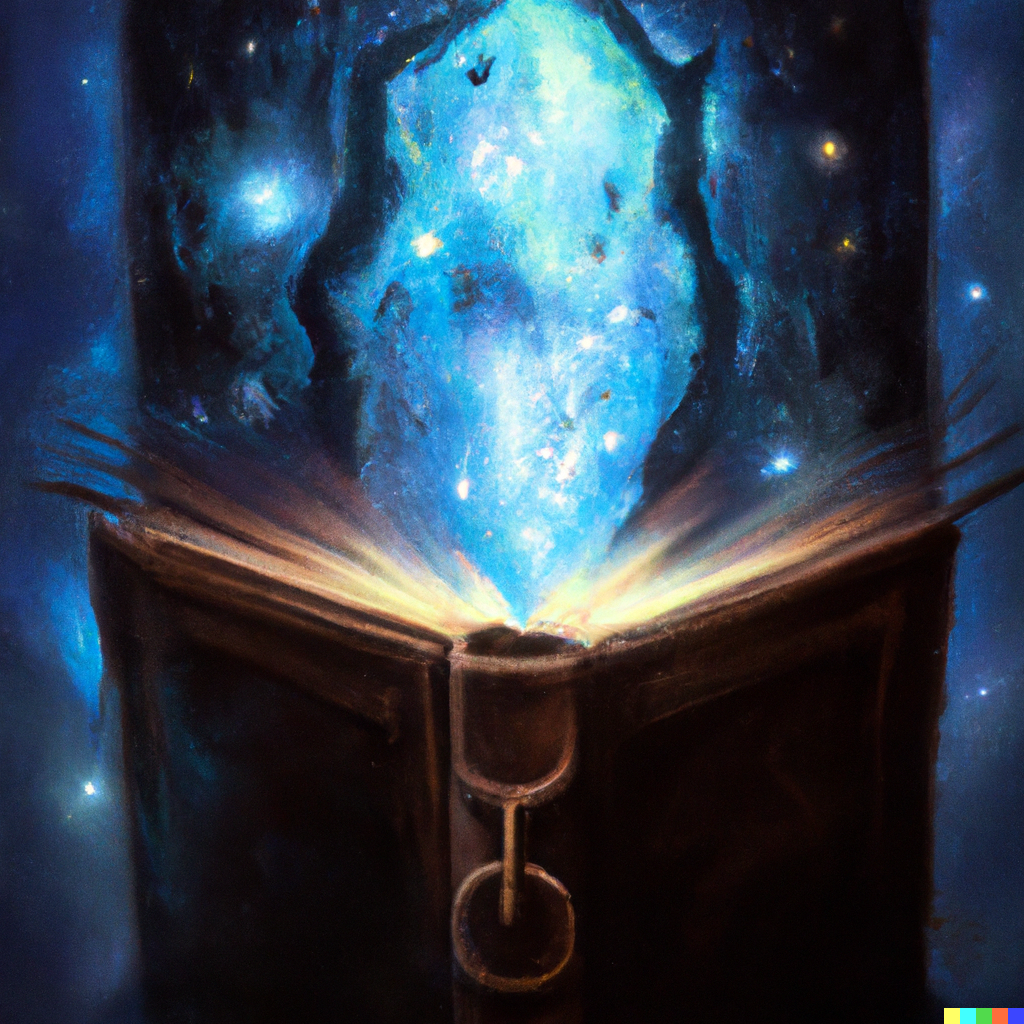
\includegraphics[width=\columnwidth]{the universe/secrets of the universe}

    There are many mysteries in the universe of Rise.
    This section gives a glimpse into some of the underlying truths, though few characters in the universe would understand such details.

    \subsection{Power Ultimately Derives From Souls}
        At a surface level, Rise seems to have a deep and fundamental divide between magical and mundane effects.
        The physical abilities of a mighty barbarian and the divine magic wielded by a cleric are generally believed to come from completely different sources.
        In truth, these are all just reflections of the ultimate source of power for everything in Rise: the soul.

        When living creatures are born, they enter existence with a new soul.
        This is the fundamental miracle of life, and no one knows where these souls come from.
        Souls in Rise have an intrinsic power, but not all souls are equal in power.
        Even the combined power of the souls inhabiting a vast colony of ants is dwarfed by the soul of a dog or cat, and that too pales in comparison to the soul of a humanoid creature like a human or elf.
        Humanoid creatures have unusually potent souls, though some rare monsters, such as dragons, have souls of similar intrinsic strength.

        \subsubsection{Transferring Souls}
            The intrinsic power of souls can be transferred.
            The simplest method of transfer is through death.
            When a predator kills its prey, the prey's soul is shattered and vulnerable in the moments after death.
            If the killer's soul is strong enough, it can ingest a fraction of the dead creature's and make its energy a part of its own soul.
            Weak-souled creatures are unable to feed on soul energy in this way.
            No matter how many rabbits a typical wolf kills, it will never gain a level.
            It is simply a wolf, and lacks the capacity to be more than that.

            Strong-souled monsters can gain a great deal of power by feeding on the souls of dead creatures.
            By repeatedly killing creatures with souls and feeding on the soul splinters emitted during death, they grow their own power.
            Likewise, an adventurer that kills a monster claims a piece of that monster's soul - including the combined power of all soul splinters the monster absorbed in its life.
            With appropriate magical rituals, it is possible to allow deities or distant creatures to feed on the soul of a dying creature.
            Demons and minor deities sometimes use this principle to feed on souls offered to them in ritual sacrifices by their cultists.

            Transferring a soul's power through death is deeply inefficient.
            Under normal circumstances, only a fraction of a soul's power can be absorbed in this way.
            Some of the soul's power splashes into the surrounding world at the location of a creature's death, where it creates or fuels natural magical phenomena in the area.
            Creatures with strong souls, like humanoid creatures, retain their sense of self and are reborn in an appropriate afterlife with the vast majority of their soul intact (see \pcref{Deities and Afterlifes}).

            A soul's power can be transferred without the inefficiency of death.
            Commonly, it is simply freely given through love and emotional connection in the form of soul motes.
            Creatures who love each other naturally share small portions of their souls with each other.
            Over time, deeply connected creatures, such as old married couples, can mix their souls so fully that they become virtually indistinguishable.

            Voluntary soul sharing does not have to be perfectly symmmetric, of course.
            Tyrants can earn soul motes through the enforced fear and subservience that they create in their underlings.
            Worship is another method of transferring soul motes, and many deities fundamentally derive power from the combined soul motes willingly given by their legions of worshippers.
            In exchange, deities can use their power to protect their worshippers, either through divinely empowered clerics or more rarely through direct intervention.
            More mundanely, adventurers who save a town from a dire threat may earn soul shards freely granted from the gratitude of its inhabitants.

        \subsubsection{Soul Motes and Splinters}
            Souls can be subdivided into lesser pieces.
            There are two forms of lesser soul pieces: motes and splinters.

            Soul motes are emitted from souls unconsciously, like light is emitted from a torch.
            It is possible for a soul that emits a large number of soul motes to diminish if it does not receive any in exchange.
            For example, a minor underling who pledges their life to an uncaring leader might give away far more soul motes than they receive in exchange.
            Most people have enough interpersonal relationships to avoid this danger, but completely isolated people who are neither loved nor hated, but simply ignored, may diminish in this fashion.
            Even with this risk, the process of emitting soul motes is not harmful or individually significant in any way.
            In addition, individual soul motes are far too small to be manipulated or used by magical effects.

            Soul splinters are created in a much more dramatic fashion.
            When a soul undergoes significant trauma that shakes its will and sense of self, it may splinter, losing a chunk of its soul.
            Of course, death is one of the greatest traumas of all, and almost all souls splinter to some degree when they die.

            Soul splinters can be consumed or manipulated in a variety of ways.
            For example, demons are formed from soul splinters that drift into the Abyss.
            Undead creatures are animated by splintering a soul that originally inhabited a corpse and using that splinter to animate the corpse.

        \subsubsection{Souls and Intrinsic Power}
            As creatures gain soul splinters and motes, they may increase their personal power, which is represented in Rise as increasing their level.
            This does not mean that a creature's level or overall combat power is directly correlated to the strength of its soul.
            A well-trained soldier will easily defeat a commoner in battle, but this does not mean that the soldier's soul is stronger.
            Bears are physically much stronger than humans, and a typical bear is higher level than a commoner, but they have much weaker souls.

            Essentially, a creature's intrinsic strength, including its special abilities, determine the baseline power for a standard adult of that species.
            For monsters, this baseline power can be far beyond an ordinary human.
            Training and experience alone can increase that power slightly, but up to a clear limit, which is generally up to three levels beyond the baseline.
            To develop beyond that point, a creature must draw power from other souls into itself.

            The strength of a creature's soul determines how much power it can incorporate from other souls.
            Creatures with a weak soul cannot master the raw energy contained within soul splinters they are exposed to, and cannot gain levels in this way by any means.
            A strong soul allows a creature to fully incorporate the energy of other souls into itself, and the strength of the soul determines the upper limit.
            For example, a dire wolf has an unusually strong soul for an animal, but it still eventually reaches a maximum level that it cannot surpass.
            Typically, only about 10\% of the humanoid population has a strong enough soul to exceed 10th level, though of course few even reach that point.
            All player characters are assumed to have have exceptionally strong souls even relative to normal humanoid creatures, and are able to reach 21st level.
            Legendary monsters of epic proportions may have still stronger souls, and be able to surpass that limit.

        \subsubsection{Mysteries of the Soul}
            The mysteries of differing soul strength have no clear and consistent explanation.
            In broad terms, the strength of a creature's soul usually correlates to its emotional and intellectual potential, as well as its force of will.
            Humanoid creatures and dragons are unusually mentally capable - not just in raw intelligence, but also in empathy, determination, and capacity for belief - and correspondingly have unusually strong souls.
            There are individual exceptions that suggest that this is not the entire dimension of what causes strong and weak souls.
            It is not uncommon for animals to have unusually strong souls for no known reason, causing them to develop over time into their ``dire'' variants.
            Dire animals, who have gained levels by feeding on soul splinters, do not seem obviously more emotionally or intellectually capable than ordinary animals.
            Perhaps there is simply an element of randomness in the creation of each new soul.

            The fundamental mysteries of souls and their sharing is not widely known in the universe of Rise.
            Individual elements of this truth are widely known, such as the observation that people can become stronger by slaying monsters, but monsters do not seem to grow dramatically in power by killing people.
            Strange phenomena can occur where death occurred, and old battlegrounds are often haunted by naturally occuring undead.
            Learned scholars may understand that the civilized species like humans seem to have unusually strong souls, and that this is related to their capacity for drastic personal growth.
            They may identify the general phenomena surrounding soul splinters, but not soul motes.

            Some powerful and unusual entities, such as deities and greater demons, know particular elements of how soul energy can be transferred.
            Greater demons are generally aware that they can feed on soul splinters from souls in evil afterlife planes as they lose their cohesion over time.
            They attempt to torment weaker souls to accelerate this breakdown, and avoid souls that are too strong to break.
            However, they are unaware of the subtler aspects of soul sharing, such as willing soul mote transfer between loved ones.
            Powerful deities know more about souls than any other entities as a result of being worshipped and maintaining the existence of their personal afterlife planes.
            In exceptionally rare occasions they may see fit to share that knowledge if it serves their purposes.

    \subsection{Soul-Fuelled Phenomena}

        The peculiar nature of soul energy causes a wide variety of strange and unique effect in the Rise universe.

        \subsubsection{Deities}
            Deities are among the most obvious phenomena that are fundamentally created by the energy of souls.
            When hordes of living creatures pay homage to the same entity, that entity can feed on that outpouring of worship and become incredibly powerful if it has a strong enough soul.
            The background of Rise is full of minor deities and demigods who either lack a sufficient base of worshippers to become a true deity or who lack a strong enough soul to effectively use the worship they receive.

            Not every powerful entity with a large amount of soul energy is a deity.
            Deities are sentient creatures that fundamentally owe their power to voluntary worship.
            Soul energy gained through voluntary transfer, including worship, is subtly different from soul energy gained through other means.
            The most notable difference is that this soul energy is easier to efficiently re-transfer to other entities.
            This makes deities more likely to share their power with select worshippers who serve their ends.
            In most societies, these empowered worshippers are called clerics.

            A deity that gains a sufficient base of worshippers can claim territory within the afterlife plane associated with its alignment.
            Deities have extraordinary power within their claimed territory, and can reshape it as they see fit.
            However, they must expend a significant amount of soul energy to maintain their territory.
            As a result, deities are always hungry to gain additional followers, and only successful deities expend the effort to claim any territory at all.

            Any souls that worship a deity will be reborn within that deity's territory in the appropriate afterlife plane, even if that plane does not match their personal alignment.
            This is both a reward for worshippers and a way for deities to accumulate soul energy.
            When a soul in an afterlife eventually loses the will to maintain its individual existence, its soul energy is absorbed by the afterlife plane it is on.
            Deities can harvest a portion of that power for themselves, though most of it still transfers to the plane as a whole.
            In addition, this allows deities to eventually reclaim the soul energy they invested in their clerics.

        \subsubsection{Nature}
            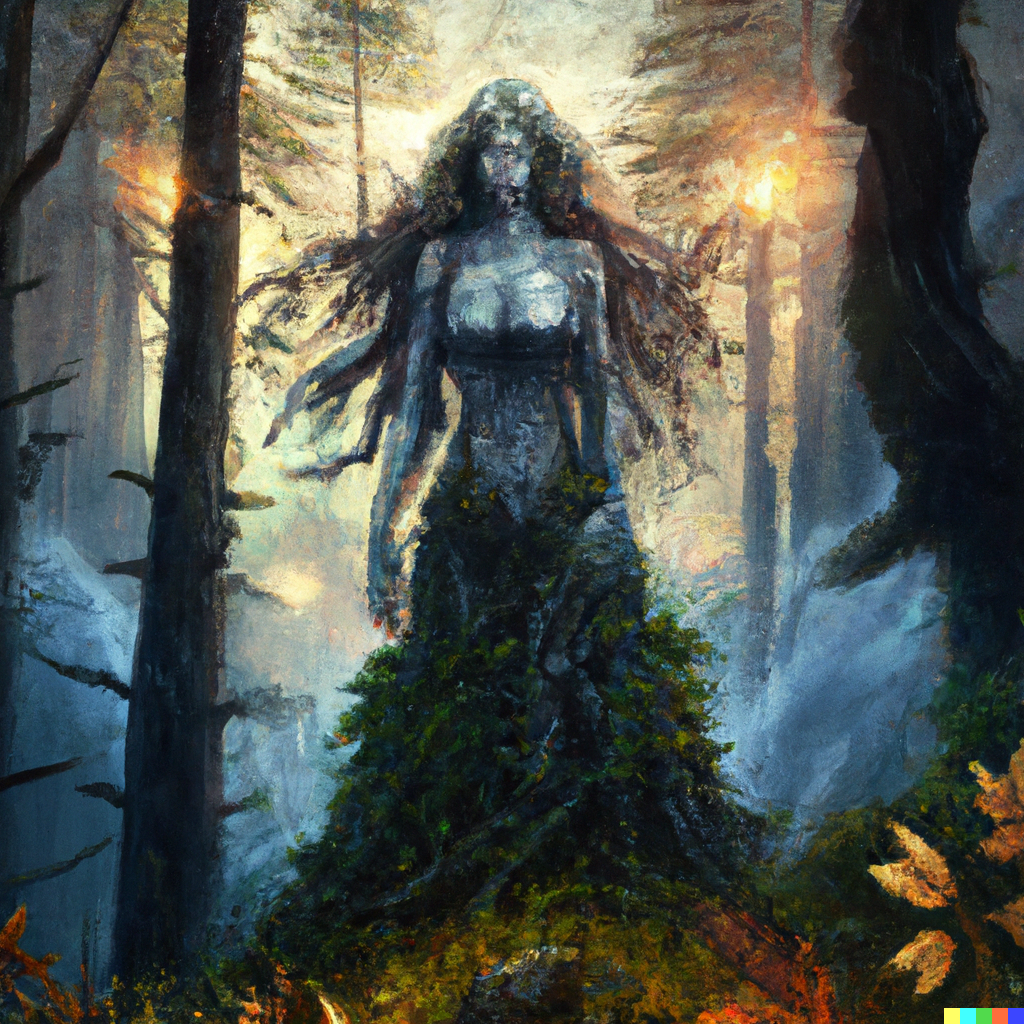
\includegraphics[width=\columnwidth]{the universe/nature}
            Nature itself has an immensely vast soul, but although people can worship Nature, it is not a deity because does not depend on mortal worship for its power.
            Nature claims the greatest tithe of every unclaimed death - every predator hunting a prey, every swatted fly.
            These souls are individually tiny.
            However, the combined soul energy released by billions of deaths over millenia dwarfs the power of any other individual entity in the Rise universe.

            Nature lacks a coherent anthropomorphic representation, and its will is almost never brought to bear in any organized way.
            Druids are granted power by Nature, but they need not agree to any particular ideology, and their usage of that power is virtually never policed or revoked by Nature itself in the way that a misbehaving cleric might be punished by their deity.
            Nature welcomes a diversity of viewpoints, for it is itself almost infinitely diverse.
            It has a wealth of power, and it does not expend soul energy maintaining territory in an afterlife plane, so it does not need to jealously hoard its gifts like deities must.
            The only druids who have had their powers revoked were a rare few who turned their powers to the explicit and intentional destruction of Nature itself.

            People who worship nature do not have any special territory in an afterlife reserved for them, since Nature claims no part of any afterlife.
            The afterlife planes are where Nature's power is weakest, and it can claim no tithe of any deaths there, since the planes themselves absorb the soul energy.
            Instead, devoted worshippers of Nature may have their souls reincarnated instead of going to a normal afterlife.
            This gift is not granted to all worshippers, and indeed many would prefer to go to a normal afterlife.

            Every plane that is not the Astral Plane an afterlife plane is a manifestation of Nature's power in some sense, and it claims deaths that occur on any of those planes.
            The four Elemental Planes - Air, Fire, Earth, and Water - are the grandest manifestations of Nature's power.

        \subsubsection{Pact Magic}
            Entities of great power can make pacts with mortals.
            In these pacts, the mortals offer their soul to the entity for a period of time after death, and the entity who becomes their soulkeeper.
            In exchange, the soulkeeper grants the mortal soul energy from its own supply.
            The soulkeeper's goal is to have the mortal gain a great wealth of its own soul energy in its life, and then to break the will of the soul while it is in the soulkeeper's clutches.
            If the soulkeeper succeeds, it gains the rare and powerful ability to feed on the mortal's entire soul.
            This is a vast wealth of soul energy compared to the normal shards extracted from death and worship, and it annihilates the mortal's soul, preventing it from travelling it to its normal afterlife.

            Successful soulkeepers can therefore amass great power.
            However, it is a risky business, much like adventuring is for mortals.
            If the mortal resists the soulkeeper's torments during its time in the afterlife, it may take its entire soul intact to its normal afterlife.
            When this happens, the soulkeeper loses the bounty of the soul, all of the soul energy it originally invested in the mortal, and time it wasted trying to break the mortal's spirit.
            This is particularly likely if the mortal dies soon after making the pact, so soulkeepers must choose their mortal partners wisely.

            Failing to break a mortal's spirit is not the worst thing that can happen to an overly successful soulkeeper.
            It may may attract attention from more powerful entities within its own plane.
            When a soulkeeper is killed, ownership of the soul is transferred to whatever killed it.
            This means that soulkeepers with active contracts - especially active contracts with mortals who are nearing death after a long life - are extremely attractive targets for anyone who wants to steal the reward of the soul.

            Demons are the most common soulkeepers.
            They are more likely than any other type of creature to meet the four main prerequisites for offering soul pacts.
            First, they have sufficient raw soul energy to make soul pacts.
            Second, they have enough understanding of magic and soul energy to transfer power through the pact.
            Third, they have the patience to wait until the mortal dies to claim their reward.
            Fourth, they have the ambition and risk tolerance to take the gamble of being a soulkeeper and risk not being able to reclaim the energy they invest.

            There is nothing that prevents a deity from becoming a soulkeeper.
            On very rare occasions, deities may make a pact and become a soulkeeper for a non-worshipper.
            Mortals that gain power in this way are called favored souls.
            However, being a soulkeeper is risky.
            Few deities would risk the possibility of losing their soul energy entirely when they could instead use that soul energy to more safely empower a cleric.
            In addition, being known for making soul pacts can discourage people from voluntarily worshipping the deity.

        \subsubsection{Ambient Magic and Magical Creatures}
            The world of Rise is full of strange creatures that have superhuman strength or magical abilities, like minotaurs and manticores.
            It is common knowledge that such creatures are typically found only in distant wilderness or in deep dungeons.
            In general, the farther you get from civilization, the more powerful the monsters in the area become, and the more likely you are to encounter strange magical phenomena.
            Small towns seem to cause a subtle warding effect, and powerful monsters in the area will typically avoid them.
            Even monsters that lack the intellectual capacity to understand complex causation chains like ``if I attack the town, they may send powerful warriors to hunt me down'' will typically avoid interacting with civilization unless necessary.

            All of this can be explained by the behavior of souls.
            The constant cycle of life and death in nature produces a great wealth of soul energy.
            Most of it is claimed by Nature itself, but some spills out at the location of each death.
            This soul energy lingers and can build up over time in the form of ambient magic.
            Many monsters can instinctively feed on this ambient magic.
            This naturally allows them to build their power to near the limit of their soul's potential by the time they are adults.

            Civilization disrupts the natural cycles of life and death, reducing the soul energy present in an area.
            Although humanoid creatures have powerful souls, they die less frequently, and the vast majority of the soul energy of their death moves with them to their afterlife.
            From the perspective of creatures that feed on ambient magic, civilized areas stand out as a dead zone.

            Since educated people in the universe of Rise can observe that monsters tend to avoid civilization if they study the phenomenon, they may have their own theories about why this is true.
            Reasonable theories that might have truth to them in some contexts could include ``monsters have evolved to instinctively avoid civilization to avoid death from monster hunters'', ``druids magically discourage monsters from entering civilization so they don't get killed'', or ``monsters have to kill other strong monsters to get stronger, so they try to avoid areas that don't have any powerful prey''.

\section{Planes}\label{Planes}
    The universe of Rise is divided into planes.
    A plane is a distinct realm of existence.
    Except for the connections between planes through planar rifts, each plane is effectively an isolated universe, and different planes can obey different fundamental laws.
    For example, the Material Plane has gravity that exerts a consistent acceleration in a single absolute direction.
    However, the Astral Plane has subjective gravity, where each creature on the plane chooses the direction that gravity pulls it in, if any.

    \subsection{General Cosmology}
        The planes of Rise are divided up into groups.

        \parhead{Primal Planes} The primal planes are manifestations of the basic building blocks of the universe.
        Each plane in this group is predominantly composed of a single element or type of energy.
        There are four primal planes: Air, Earth, Fire, and Water.

        \parhead{Aligned Planes} The four aligned planes are manifestations of the four alignments.
        The Celestial Heavens is good-aligned, the Abyss is evil-aligned, Ordus is law-aligned, and Discord is chaos-aligned.

        When mortal creatures die, their souls travel to an appropriate location on an aligned plane, where they gain new planeforged bodies and live again.
        If they pledged their soul to a deity in life, that deity can take ownership over their soul in death, and the soul is reborn within that deity's territory and under their protection.
        Otherwise, they appear on the aligned plane that most closely reflects their primary alignment in life.

        For details about aligned planes, see \pcref{Aligned Planes}.

        \parhead{Nexus Planes} The nexus planes are composite planes with a number of distinct environments and filled with creatures of myriad alignments.
        Nexus planes comprise the majority of civilization across all planes.
        They do not have their own unique planar essence, and no planar creatures are native to nexus planes.
        There are two nexus planes: the Material Plane and the Astral Plane.

        \parhead{Demiplanes} These planes are small, fragmentary realms that are greatly limited in their scope.
        There is no specific list of demiplanes, and they share few common properties.
        Most demiplanes were created for particular purposes by beings of great power, though some simply came into existence through unknown means.

    \subsection{Planar Rifts}\label{Planar Rifts}
        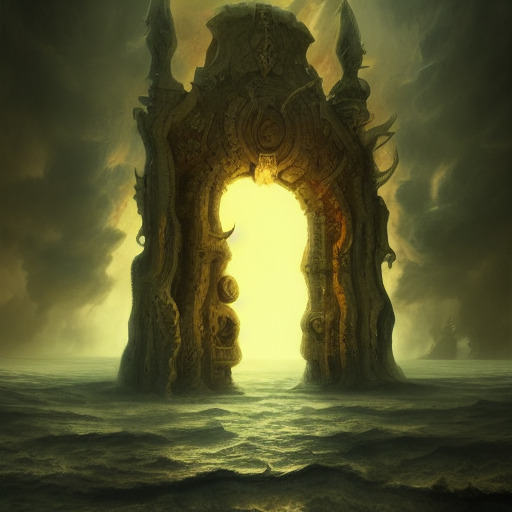
\includegraphics[width=\columnwidth]{the universe/planar rifts}
        Normally, there are boundaries between different planes that prevent direct passage between them.
        However, planar rifts are places where these boundaries have weakened, making interplanar travel easier.
        A planar rift joins a specific location on one plane to a specific location on a different plane.
        Most planar rifts lead to and from the Astral Plane, which is the space between the other planes (see \pcref{The Astral Plane}).

        Most planar rifts still require the use of magic, such as the \spell{plane shift} ritual, to actually cross between planes.
        Some especially large rifts enable physical travel between planes without the use of any magic.

    \subsection{Planar Traits}
        \subsubsection{Gravity Direction}
            The direction of gravity on a plane can take one of the following forms:
            \begin{itemize}
                \item Fixed Gravity: Gravity points in a fixed direction and with a fixed strength at all locations on the plane.
                    Almost all planes with a fixed gravity have a perfectly flat surface.
                \item Absolute Directional Gravity: Gravity points in a consistent direction according to a rule that applies equally to everything on the plane, but which is not in a fixed direction.
                    For example, a plane filled with floating spheres where gravity always points towards the closest sphere has absolute directional gravity.
                \item Subjective Gravity: Each creature on the plane chooses the direction of gravity for that creature.
                    The plane has no gravity for unattended objects and nonsentient creatures.
                    A creature on the plane can make use the \textit{control gravity} ability as a minor action.
                    \begin{activeability}{Control Gravity}
                        \rankline
                        Make a Willpower check with a difficulty value of 10.
                        Success means that you choose the direction of gravity that applies to you on the current plane.
                        Alternately, you can choose for gravity to not apply to you.

                        Failure means you gain a \plus2 bonus to the next \textit{control gravity} ability you use on this plane.
                        This bonus stacks with itself and lasts until you succeed at a \textit{control gravity} ability on this plane.
                    \end{activeability}
            \end{itemize}

        \subsubsection{Gravity Strength} The strength of gravity on a plane can take one of the following forms:
            \begin{itemize}
                \item Normal Gravity: Gravity is about the strength of Earth.
                \item No Gravity: There is no gravity on the plane.
                    The range limits of ranged weapons are quadrupled.
                    % TODO: what additional effects are there?
                \item Light Gravity: Gravity is about half the strength of Earth.
                    % Should there be check penalties?
                    The weight of all items is halved.
                    The range limits of ranged weapons are doubled.
                \item Heavy Gravity: Gravity is about twice the strength of Earth.
                    Creatures take a \minus2 penalty to Strength and Dexterity-based checks.
                    The weight of all items is doubled.
                    The range limits of ranged weapons are halved, to a minimum of 5 feet.
                    % TODO: falling damage
                \item Extreme Gravity: Gravity is about four times the strength of Earth.
                    Creatures take a \minus4 penalty to Strength and Dexterity-based checks.
                    The weight of all items is quadrupled.
                    The range limits of ranged weapons are reduced to one quarter of the normal value, to a minimum of 5 feet.
                    % TODO: falling damage
            \end{itemize}

        \subsubsection{Light} Various planes are illuminated in different ways.
            \begin{itemize}
                \item Fixed Source: There is a single constant source of light on the plane.
                \item Mobile Source: There is a single source of light on the plane that moves around it, illuminating different parts of the plane at different times.
                \item None: There is no natural source of light on the plane.
                    Other sources of light, such as torches, function normal.
            \end{itemize}

        \subsubsection{Limits} The behavior of a plane at its limits can vary widely.
            Some planes have different behaviors at different limits depending on their shape.
            \begin{itemize}
                \item Astral Gate: If you reach the limits of the plane, you find a planar gate to the Astral Plane.
                \item Barrier: If you reach the limits of the plane, you find an impassable barrier.
                    The barrier takes the form of a substance relevant to the plane's nature.
                    It may be possible to dig tunnels into the barrier to some depth, but there is nothing behind the barrier.
                    As you progress past the limit, the barrier becomes increasingly difficult to break through, and eventually it becomes completely impenetrable.
                \item Looped: If you go beyond the limits of the plane, you wrap around to the opposite side of the plane.
                    There is no obvious transition point or perception of transportation when this occurs - the shape of the plane simply connects to itself.
                    On very small planes, this can allow you to see your own back, though looped planes of that size are rare.
                \item Infinite: The plane has no limits. This is extremely rare.
            \end{itemize}

        \subsubsection{Planar Connectivity}
            Different planes have different degrees of connection to other planes.
            \begin{itemize}
                \item Isolated: The plane is difficult to reach or leave.
                    It has no permanent planar rifts, and temporary rifts are rare or nonexistent.
                \item Stable Connected: The plane has multiple permanent planar rifts.
                    However, temporary rifts are rare.
                \item Unstable Connected: The plane has no permanent planar rifts, but temporary rifts are common.
                \item Conduit: The plane has a large number of permanent planar rifts, and temporary rifts are common.
            \end{itemize}

        \subsubsection{Shape} The shape of a plane defines the shape of its core surface, and what happens if you travel beyond that surface.

            \begin{itemize}
                \item Flat Surface: The plane consists of a flat surface generally made of earth or similar material.
                    Most activity and civilization on the plane happens on this surface.
                    It is usually possible to construct tunnels into a flat surface plane to some depth, depending on the size of the plane.
                \item Hollow Sphere: The plane consists of a hollow sphere with an outer boundary generally made of earth or similar material.
                    Most activity and civilization on the plane happens on the inner surface of the sphere or in the vast open space between.
                    Some hollow sphere planes have an outer surface that can also be accessed, but in most planes it is impossible to leave the interior of the sphere.
                \item Solid Sphere: The plane consists of a solid sphere generally made of earth or similar material.
                    Most activity and civilization on the plane happens on the surface of the sphere.
                    It is possible to construct tunnels into a solid sphere plane, but it may become increasingly difficult to traverse the plane as you approach the center of the sphere.
                    In general, the limit of a solid sphere plane is located at ten times the radius of the plane's primary sphere.
                \item Uniform: The plane has no well-defined surface or ground layer.
                    Some uniform planes have no ground or solid obstacles, while others are composed almost entirely of ground and firmament.
                    Uniform planes almost always still have limits of some kind.
            \end{itemize}

    \subsection{Planeforged Creatures}
        A planeforged is a type of creature that is fundamentally composed of the essence of one or more planes.
        The vast majority of planeforged creatures are composed of only a single plane.
        When a planeforged dies, its essence returns to its native plane or planes.
        Weak planeforged lose their independent identity and become part of the core composition of the plane once more.
        Strong planeforged can retain their identity and reform from that raw material given time, making them difficult or impossible to kill completely.
        In either case, planeforged cannot be resurrected by soul-based magic such as the \spell{resurrection} spell.

            % TODO: morphicness, alignment, magic

\section{Plane Descriptions}

    \subsection{Primal Planes}

        \subsubsection{The Plane of Air}
        The Plane of Air is a a soaring landscape unencumbered by gravity or ground.
        The vast expanses of empty air are littered with clouds and unpredictable winds.
        Any inhabitants of the plane must adapt to a highly mobile lifestyle.
        A number of towns and structures have been built in the plane using raw materials brought from other planes.
        They sail through the air at the whims of the wind, and are occasionally battered by intersections with other wind streams.

        The Plane of Air has the following planar traits:
        \begin{itemize}
            \item Gravity strength: No gravity
            \item Light: Fixed source, from a sun outside the limits of the plane
            \item Limits: Barrier, formed from wind currents which push back with such force that nothing can travel far.
            \item Planar connectivity: Unstable connected
            \item Shape: Hollow sphere with a radius of about 2,000 miles.
        \end{itemize}

        \subsubsection{The Plane of Earth}
        The Plane of Earth is a titanically large body of earth and stone.
        A labyrinthine series of mostly airless tunnels weave their way through the plane, connecting the few cities.
        The plane is a major source of valuable gems, diamonds, and rare metals like mithral, but the dense rock and airless environment make successful mining difficult.
        In addition, earthquakes periodically reshape the environment by collapsing old tunnel systems and constructing new ones.
        Some cities have been carved out in vast underground rooms reinforced to survive the earthquakes.

        The Plane of Earth has the following planar traits:
        \begin{itemize}
            \item Gravity direction: Fixed
            \item Gravity strength: Normal
            \item Light: None, though cities tend to be well-lit
            \item Limits: Barrier, formed from increasingly dense rock that eventually becomes so hard that no known material or magic can damage it.
            \item Planar connectivity: Stable connected
            \item Shape: Hollow sphere with a radius of about 500 miles.
        \end{itemize}

        \subsubsection{The Plane of Fire}
        The Plane of Fire is an endless searing inferno.
        The plane's essence is highly combustible, allowing fires to burn indefinitely without any obvious fuel.
        However, the intensity of flames on the plane are highly uneven, as the plane generates fuel in various locations that shift over time.
        Some pockets on the surface are devoid of natural fuel, allowing the allow the construction of trading hubs where the few inhabitants of the plane who are not naturally immune to fire can survive.

        The Plane of Fire has the following planar traits:
        \begin{itemize}
            \item Gravity direction: Fixed
            \item Gravity strength: Normal
            \item Light: None, though the constant fires provide sufficient illumination in most locations on the plane
            \item Limits: Barrier, formed from fires which burn so fiercely that further travel becomes physically impossible, even for creatures immune to fire.
            \item Planar connectivity: Unstable connected
            \item Shape: Flat surface, in a disc with a radius of about 2,000 miles.
        \end{itemize}

        \subsubsection{The Plane of Water}
        The Plane of Water is an impossibly vast ocean.
        Powerful currents sweep through the ocean, but much of it is calm, and many forms of aquatic life abound in the water.
        The Plane of Water is the most densely populated Primal Plane, both by sentient creatures and monsters.
        Magnificant underwater cities are carved from huge rocks that float peacefully suspended in the water.
        Though there is no sun, simple creatures akin to plankton form the base of the food chain by feeding directly on the plane's essence.

        The Plane of Water has the following planar traits:
        \begin{itemize}
            \item Gravity strength: No gravity
            \item Light: None, though bioluminescent creatures like plankton are extremely common, making many parts of the plane well-lit
            \item Limits: Barrier, formed from water currents which push back with such force that nothing can travel far.
            \item Planar connectivity: Stable connected
            \item Shape: Hollow sphere with a radius of about 1,000 miles.
        \end{itemize}

        \subsection{Aligned Planes}\label{Aligned Planes}

            \subsubsection{The Celestial Heavens}
                The Celestial Heavens are beautiful and majestic.
                Mountains rise dramatically out of misty clouds, trees are massive and laden with delicious fruit, and buildings surpass the wildest dreams of mortal architects.
                A serene blue sky gives way to a night so lit by stars that it is almost as bright as the day.

            \subsubsection{The Abyss}
                The Abyss is a hellscape of fire, brimstone, and distant screaming.
                With the exception of the great palaces of demon princes, the buildings that exist are designed for defense rather than aesthetics.
                The terrain is typically rocky and dull, and most of the color belongs to carcasses left behind after violent battles.

                All manner of nightmarish creatures stalk the Abyss.
                The best known of these creatures are demons and devils.
                Demons are formed when mortal souls are splintered by trauma.
                The soul splinters drift into the Astral Plane, and from there are guided to the Abyss by ancient astral currents.
                When they arrive in the Abyss, its planar essence envelops them in new planeforged body, much like dead souls gain new bodies in their proper afterlife.

                Newly formed demons, known as demonspawn, are barely functional creatures.
                They are driven entirely by the primal emotion that separated the soul splinter from its original soul, such as rage, grief, or pain.
                This makes them functionally insane, and they are almost always driven to lash out at everything around them.
                Rage-born demons violently attack anything they see, pain-born demons try to lessen their pain by sharing it, and so on.
                When they succeed in their attacks, they can feed on the trauma they inflict, strengthening their soul.
                Unfortunately, this does not generally make them more sane, since they only feed on the same urges that created them.

                Demonspawn instinctively avoid attacking other demonspawn, since they can find no gratification for their urges in attacking such small, broken souls.
                Instead, they hunt creatures with complete souls, which generally means attacking the afterlife bodies of evil-aligned creatures who went to the Abyss for their afterlife.
                The greatest feast, however, comes from attacking mortal souls, which are much easier to splinter.
                Demonic incursions into other planes are devastating but fortunately rare.

                Unlike demons, devils are native to the Abyss itself.
                They are far more intelligent and organized than demons, but also far less numerous.
                Devils rule vast territories within the Abyss, using demons as their foot soldiers to protect and enlarge their territorial claims.

                The only competition with devils for rulership of the Abyss comes from the evil deities and greater demons.
                Evil deities are fairly simple to deal with.
                They have absolute dominion over their own territory, so invading their lands is pointless.
                In addition, since their territorial limits come from their divine power rather than force of arms, they have little ability to expand or even exert significant influence outside of their own lands.
                As a result, devils and greater demons alike mostly ignore the deities.

                Greater demons are much more troublesome.
                On rare occasions, demonspawn are so successful in their attacks that they claim soul splinters outside the scope of their original urges.
                This typically happens when demons find and break mortal souls.
                When this happens, the demonspawn gains a more complete soul, and becomes a little more sane.
                Often, this simply entices other demonspawn to attack and destroy the wayward demon.
                However, if the demon survives the attacks from its allies and repeats this process, it can grow in power.

                Demons who have expanded their soul beyond a single soul splinter are called greater demons.
                Eventually, the demon can gain something resembling a complete soul from all of the splinters it has collected, making it a demon prince.
                Though more sane and functional than demonspawn, these more developed demons are no less evil.
                Both greater demons and demon princes have enough skill with splintering and manipulating souls to make pacts with warlocks.
                In addition, demon princes have the power to command armies of demonspawn and greater demons, allowing them to claim territory like devils do.

            \subsubsection{Ordus}
                Ordus is a masterpiece of logical organization.
                It is the most consistently civilized of the aligned planes, and the cities are exquisitely planned.
                However, laws are enforced with extreme severity.
                Outside of the cities, even the natural territories are cleanly and simply divided.
                A forest of evenly spaced trees might border a field in a sharp, clean transition along a perfectly straight line.

            \subsubsection{Discord}
                Discord is a wild maelstrom.
                Much of the plane can be freely reshaped with only minimal force of will.
                By working together, its inhabitants can create vast cities from thin air, though they can be destroyed with similar ease.
                Beyond the shaped spaces, the terrain is constantly changing.
                A field might grow trees that are consumed by a forest fire and then fall into chasms newly formed by an earthquake in a matter of minutes.

    \subsubsection{Nexus Planes}

        \parhead{The Material Plane}\label{The Material Plane}
        The Material Plane is the plane that most Rise adventures begin on.
        The surface of the plane is a massive sphere with a radius of about 4,000 miles.
        It is the most familiar to most humanoid creatures.

        The Material Plane has the following planar traits:
        \begin{itemize}
            \item Gravity direction: Absolute Directional, pointing to the center of the sphere
            \item Gravity strength: Normal
            \item Light: Mobile Source, from a sun and moon outside of the plane's limits
            \item Limits: Looped
            \item Planar connectivity: Isolated
            \item Shape: Solid Sphere, with a radius of about 4,000 miles.
        \end{itemize}

    \parhead{The Astral Plane}\label{The Astral Plane}
        The Astral Plane is the space between the other planes.
        It is a necessary intermediate destination for virtually all planar journeys, as all planar rifts lead to and from the Astral Plane.
        Most activity on the Astral Plane occurs in a space called the Inner Astral Plane, a massive but finite region where all planar rifts on the Astral Plane appear.
        % Are there any other infinite planes?
        However, unlike all other planes, the Astral Plane has no known limits to its extent, and may in fact be infinite.
        The area outside the Inner Astral Plane is known as the Deep Astral Plane, and few venture into those sparsely populated realms.
        % This should be more clearly defined
        The Deep Astral Plane has magical turbulence that interferes with long-range communication and transportation magic, making exploration difficult.

        The Astral Plane has the following planar traits:
        \begin{itemize}
            \item Directional gravity: Subjective
            \item Gravity strength: Normal
            \item Light: Fixed Source, from the infinite reaches of the Deep Astral Plane
            \item Limits: Infinite
            \item Planar connectivity: Conduit
            \item Shape: Uniform
        \end{itemize}

\section{Creatures and Objects}
    In the world of Rise, creatures and objects are meaningfully different.
    Many abilities only affect creatures or objects.
    The difference between a creature and an object is defined as being agency.
    Creatures have agency, and objects do not.
    This is not the same as sentience or life, which either creatures or objects may have.

    For example, skeletons are nonsapient, nonliving creatures.
    Conversely, trees are nonsapient, living objects.
    Some rare magic items can be made intelligent by magic, making them sapient, nonliving objects.
    Some unintelligent animals and magical beasts like ants and giant spiders are nonsapient, living creatures.

    There are two types of creatures that break these rules: constructs and indwelt.

    % TODO: should constructs regain hit points and DR when they rest?
    \subsection{Constructs}\label{Constructs}
        Constructs are creatures that are made of nonsapient matter.
        Their inanimate bodies are given a semblance of life and sentience by some form of magic.
        Like other creatures, they can move and follow instructions.
        However, they lack agency and cannot make the independent decisions.
        They are \trait{mindless}, making them immune to \abilitytag{Compulsion} and \abilitytag{Emotion} effects.
        Constructs lack a soul and cannot be resurrected by any means if they are destroyed.

        Constructs are considered to be both creatures and objects, and are affected by abilities which affect either.
        They are not alive, and they do not need to eat, drink, or sleep.
        They are always considered to be \glossterm{attended} by themselves, so they are never affected by abilities that only affect unattended objects, even while unconscious.

        Constructs are not affected by the Medicine skill, and do not normally remove \glossterm{vital wounds} when they take a \glossterm{long rest}.
        Instead, their vital wounds must be repaired manually.
        This functions like like \ability{accelerate recovery} ability from the Medicine skill, except that it uses an appropriate Craft skill and raw materials appropriate to the construct's construction.

    \subsection{Indwelt}\label{Indwelt}
        Indwelt are creatures that are made of nonsapient matter.
        Their inanimate bodies are awakened to life by connection to an external soul.
        They have agency and true intelligence like normal creatures.

        The soul of an indwelt has no connection to the matter that composes its body.
        This contrasts with undead, which always maintain a connection between a body and its original soul.
        As a result, an indwelt's connection to its physical body is weak.
        If an indwelt is killed, it can be resurrected, but its previous body is not considered its corpse in the same way that a human's dead body is.
        This means it cannot be resurrected by magic that uses the corpse of the deceased creature.

        Indwelt are considered to be both creatures and objects, and are affected by abilities which affect either.
        They are alive if their base matter is alive, but not if their base matter is dead or inorganic.
        If they are alive, they need to eat, drink, and sleep.
        They are always considered to be \glossterm{attended} by themselves, so they are never affected by abilities that only affect unattended objects, even while unconscious.
